\documentclass[13pt,aspectratio=169,t,xcolor=table]{beamer}
\usepackage[utf8]{inputenc}

\usepackage{booktabs} 
\usepackage{subcaption}
\usepackage{adjustbox}
\usepackage{adjustbox}

\usetheme{Ufg}

%-------------------------------------theorems--------------
\newtheorem{conj}{Conjetura}
\newtheorem{defi}{Definição}
\newtheorem{teo}{Teorema}
\newtheorem{lema}{Lema}
\newtheorem{prop}{Proposição}
\newtheorem{cor}{Corolário}
\newtheorem{ex}{Exemplo}
\newtheorem{exer}{Exercício}

\setbeamertemplate{theorems}[numbered]
\setbeamertemplate{caption}[numbered]

%-------------------------------------------------------------%
%----------------------- Primary Definitions -----------------%

% This command set the default Color, is also possible to choose a custom color
\setPrimaryColor{TorVergataGreen} 

% First one is logo in title slide (we recommend use a horizontal image), and second one is the logo used in the remaining slides (we recommend use a square image)
\setLogos{lib/logos/LOGO-ATENEO_BIANCO_20230308.png}{lib/logos/LOGO-ATENEO_Variante1_Bianco_20230307.png} 


% -------------------------------------- Title Slide Information
\begin{document}
\title[Inf UFG]{Hard Disk Failure Data Processing}
\subtitle{Corso di Sistemi ed Architetture per Big Data}

\author{
    \begin{tabular}{c c}
    Luca Falasca & Matteo Conti \\
    0334722 & 0323728
  \end{tabular}
}

\institute[UFG] % (optional)
{
  Progetto 1 - Batch processing
}
\date{2024}
%-----------------------The next statement creates the title page.
\frame[noframenumbering]{\titlepage}


%------------------------------------------------Slide 1
\setLayout{vertical} % This command define the layout. 'vertical' can be replace with 'horizontal', 'blank, 'mainpoint', 'titlepage'

\begin{frame}
    \frametitle{Indice}
    \tableofcontents
\end{frame}
%---------------------------------------------------------

%---------------------INTRODUZIONE---------------------------
\section{Introduzione}
%---------------------------------------------------------Slide 2
\setLayout{mainpoint}
\setBGColor{TorVergataGreen}
\begin{frame}{}
    \frametitle{Introduzione}
\end{frame}
%---------------------------------------------------------

\subsection{Obbiettivi}
%---------------------------------------------------------Slide 3
\setLayout{vertical}
\begin{frame}{Obbiettivi}
    Il progetto verte sull'analisi di un dataset contenente dati riguardanti il monitoraggio di dischi rigidi installati all'interno di un cluster di server gestito da un cloud provider, in particolare si vuole: 
    \vspace{0.3cm}
    \begin{itemize}
        \item Realizzare una pipeline di elaborazione dati
        \item Eseguire le query richieste dalla specifica
        \item Visualizzare i risultati
        \item Analizzare le performance ottenute con i formati dati CSV e Parquet
    \end{itemize}
    \vspace{0.3cm}
    \begin{figure}
        \raggedright
        \hspace{2cm}
        
\includegraphics[width=.7\textwidth]{res/intro_icon.png}
    \end{figure}
\end{frame}
%---------------------------------------------------------

%---------------------------------------------------------Slide 4
\subsection{Dataset}
\setLayout{vertical}
\begin{frame}{Dataset}
    Il dataset fornito è una versione ridotta di quello presentato nel Grand Challenge della conferenza ACM DEBS 2024. Delle numerose colonne presenti nel dataset, ne verranno selezionate
    solamente cinque, in particolare:
    \begin{itemize}
        \item \textit{date}: data della misurazione nel formato 'YYYY-MM-DD'
        \item \textit{serial\_number}: identificativo del disco rigido
        \item \textit{model}: modello del disco rigido
        \item \textit{s9\_power\_on\_hours}: tempo di accensione del disco rigido in ore
        \item \textit{vault\_id}: identificativo del gruppo di storage server a cui il disco rigido appartiene
        \item \textit{failure}: flag che indica se il disco rigido ha subito una failure o meno
    \end{itemize}
\end{frame}
%---------------------------------------------------------

%---------------------PIPELINE---------------------------
\section{Pipeline}
%---------------------------------------------------------Slide 5
\setLayout{mainpoint}
\setBGColor{TorVergataGreen}
\begin{frame}{}
    \frametitle{Pipeline}
\end{frame}
%---------------------------------------------------------

%---------------------------------------------------------Slide 6
\setLayout{vertical}
\begin{frame}{Pipeline}
    La pipeline di elaborazione dati è stata containerizzata e deployata tramite docker compose ed è composta da cinque componenti:
    \begin{itemize}
        \item Data ingestion
        \item Data storage
        \item Data processing
        \item Analytical data storage
        \item Data visualization
    \end{itemize}
    \begin{adjustbox}{margin=0.5cm 0cm 0cm 0.58cm, center} % left, bottom, right, top 
        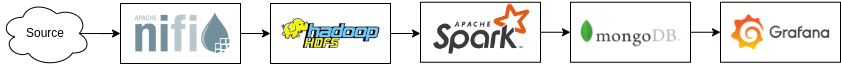
\includegraphics[width=.99\textwidth]{res/pipeline.png}
    \end{adjustbox}
\end{frame}
%---------------------------------------------------------

\subsection{Data ingestion}
%---------------------------------------------------------Slide 7
\begin{frame}{Data ingestion-Apache NiFi}
    Per la data ingestion è stato utilizzato il framework Apache NiFi, il quale si occupa di:
    \begin{columns}
        \column{0.5\textwidth}
            \begin{minipage}[b]{1\textwidth}
                \begin{itemize}
                    \item Ricevere tramite HTTP il file CSV contenente i dati
                    \item Filtrare i dati
                    \item Memorizzare i dati su HDFS in formato Parquet e CSV
                \end{itemize}
            \end{minipage}
        \column{0.5\textwidth}
            \begin{minipage}{1\textwidth}
                \begin{adjustbox}{margin=0cm 0cm 1.7cm 0cm, center} % left, bottom, right, top
                    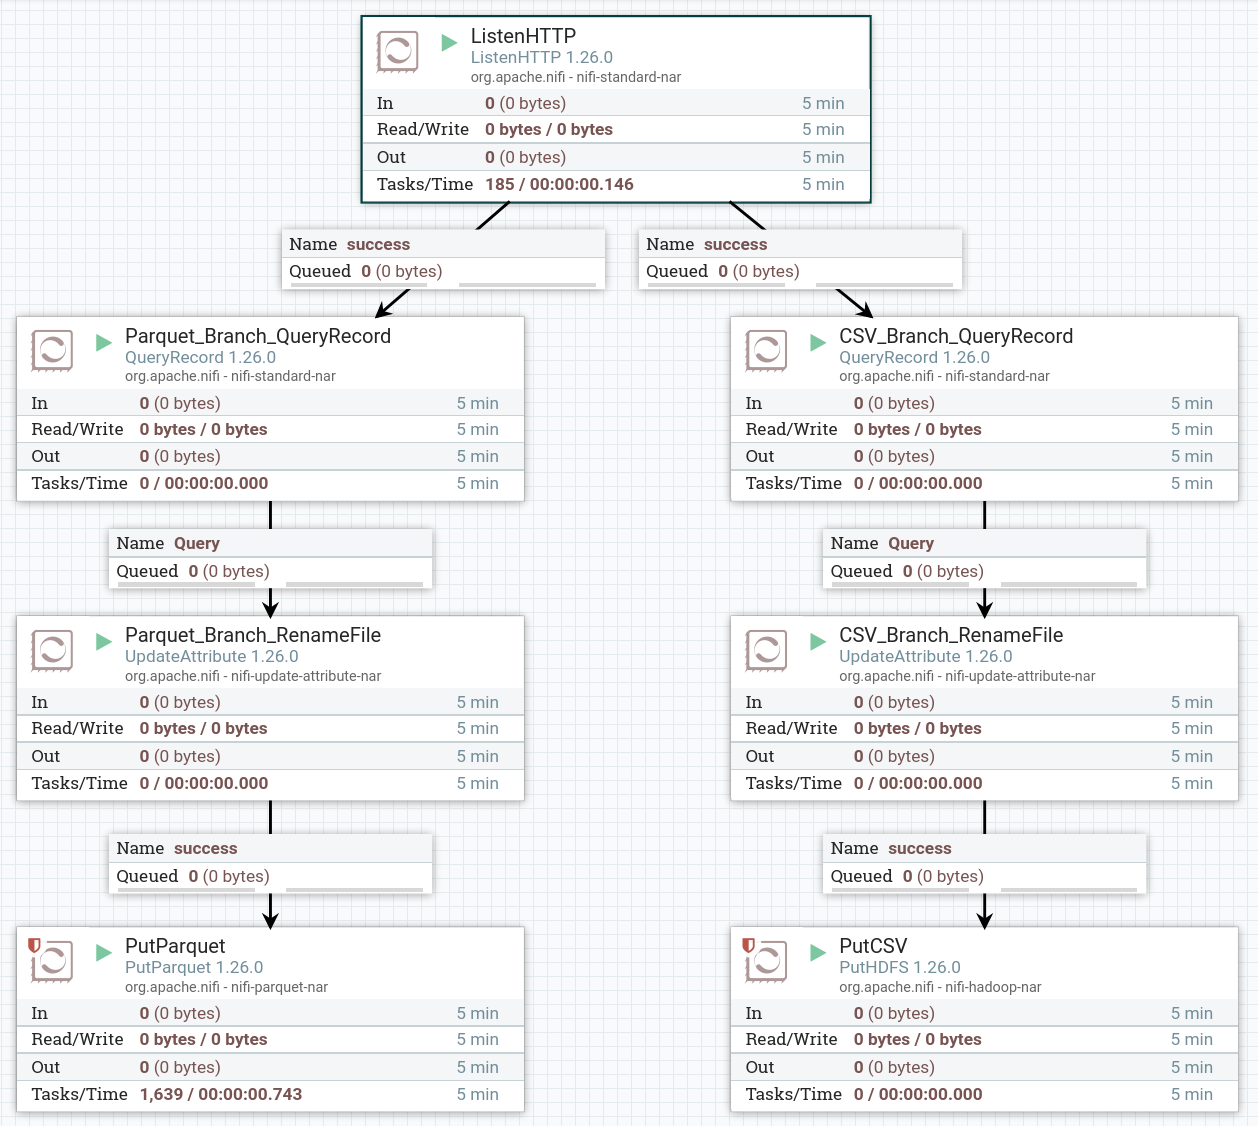
\includegraphics[width=1\textwidth]{res/nifi_flow.png}
                \end{adjustbox}
            \end{minipage}
    \end{columns}
\end{frame}
%---------------------------------------------------------

\subsection{Data storage}
%---------------------------------------------------------Slide 8
\begin{frame}{Data storage-HDFS}
    Per lo storage del dataset filtrato è stato utilizzato HDFS, non è stata utilizzata una particolare struttura del filesystem, in particolare i dati sono stati memorizzati nella root directory
    \begin{adjustbox}{margin=0cm 0cm 0cm 0.7cm, center} % left, bottom, right, top
        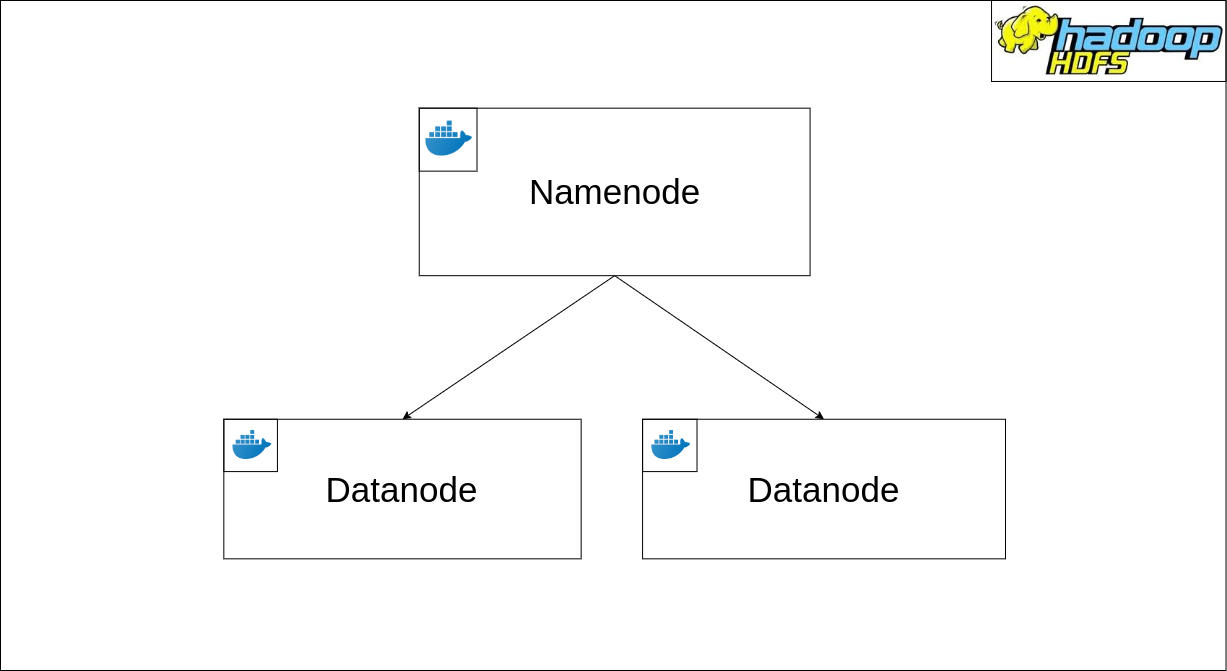
\includegraphics[width=.6\textwidth]{res/hdfs_cluster.png}
    \end{adjustbox}
\end{frame}
%---------------------------------------------------------

\subsection{Data processing}
%---------------------------------------------------------Slide 9
\begin{frame}{Data Processing-Apache Spark}
    \begin{columns}
        \column{0.5\textwidth}
            Per il processamento delle query è stato utilizzato \textbf{Apache Spark}
        \column{0.5\textwidth}
            \begin{minipage}{0.5\textwidth}
                \raggedleft
                
\includegraphics[width=.9\textwidth]{res/spark_icon.png}
            \end{minipage}
    \end{columns}
    \vspace{0.5cm}
    \begin{itemize}
        \item Cluster formato da 1 nodo master e 4 nodi worker
        \item Replicazione docker compose
    \end{itemize}
    \begin{adjustbox}{margin=0.5cm, center}
        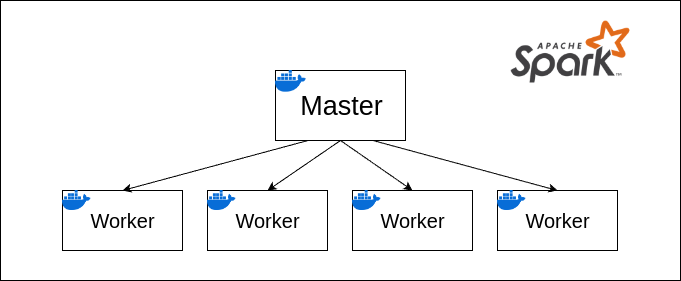
\includegraphics[width=0.7\textwidth]{res/spark_cluster.png}
    \end{adjustbox}
\end{frame}
%----------------------------------------------------------

%---------------------------------------------------------
\begin{frame}{Data Processing}
    Considerazioni:
    \begin{itemize}
        \item Ogni query è stata eseguita sia in Parquet che in CSV
        \item Standardizzazione dell'esecuzione con show()
        \item Utilizzo di DataFrame per la manipolazione dei dati
    \end{itemize}
    \vspace{1cm}
    \begin{columns}
        \column{0.5\textwidth}
            \begin{minipage}{0.3\textwidth}
                \begin{adjustbox}{margin=4cm 0cm 0cm 0cm, center}
                    
\includegraphics[width=1\textwidth]{res/csv.png}
                \end{adjustbox}
            \end{minipage}
        \column{0.5\textwidth}
        \begin{minipage}{0.5\textwidth}
            \begin{adjustbox}{margin=0cm 0cm 0.8cm 0cm, center}
                
\includegraphics[width=1\textwidth]{res/parquet.png}
            \end{adjustbox}
        \end{minipage}
    \end{columns}
\end{frame}
%----------------------------------------------------------

%--------------------------------------------------------- Slide 10
\begin{frame}{Data Processing-Query 1}
    \textbf{Q1:} calcolare per ogni giorno, per ogni vault, il numero totale di fallimenti, in particolare determinare la lista di vault che hanno subito esattamente 4, 3 e 2 fallimenti
    \begin{adjustbox}{margin=0cm 0cm 0cm 2cm, center}
        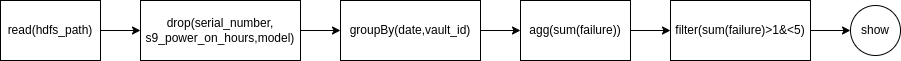
\includegraphics[width=1\textwidth]{res/query1_dag.png}
    \end{adjustbox}
\end{frame}
%---------------------------------------------------------

%---------------------------------------------------------Slide 11
\begin{frame}{Data Processing-Query 2}
    \textbf{Q2.1:} 
    Calcolare la classifica dei 10 modelli di hard disk che hanno subito il maggior numero di fallimenti, riportando il modello di hard disk e il numero totale di fallimenti subiti dagli hard disk di quello specifico modello\\ 
    \vspace{0.2cm}
    \textbf{Q2.2:} 
    Calcolare la classifica dei 10 vault che hanno registrato il maggior numero di fallimenti riportando, per ogni vault, il numero di fallimenti e la lista (senza ripetizioni) dei modelli di hark disk soggetti ad almeno un fallimento
    \begin{adjustbox}{margin=0cm 0cm 0cm 0.5cm, center}
        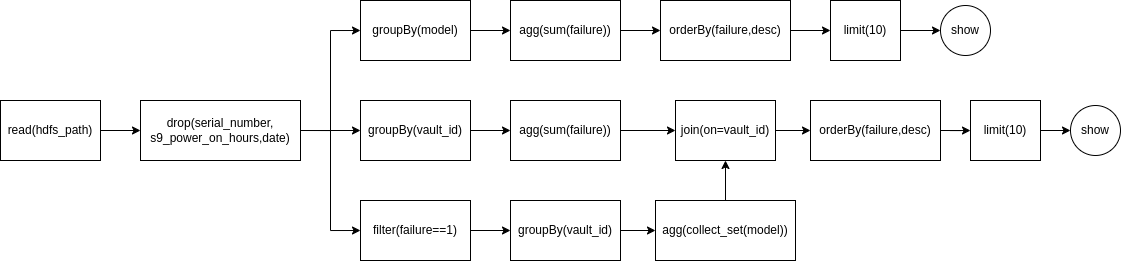
\includegraphics[width=1\textwidth]{res/query2_dag.png}
    \end{adjustbox}
\end{frame}
%----------------------------------------------------------

%---------------------------------------------------------Slide 12
\begin{frame}{Data Processing-Query 3}
    \textbf{Q3:} Calcolare il minimo, 25-esimo, 50-esimo, 75-esimo percentile e massimo delle ore di funzionamento hark disk che hanno subito fallimenti e degli hard disk che non hanno subito fallimenti, indicando anche il numero totale di eventi utilizzati per il calcolo delle statistiche
    \begin{adjustbox}{margin=0cm 0cm 0cm 0.5cm, center}
        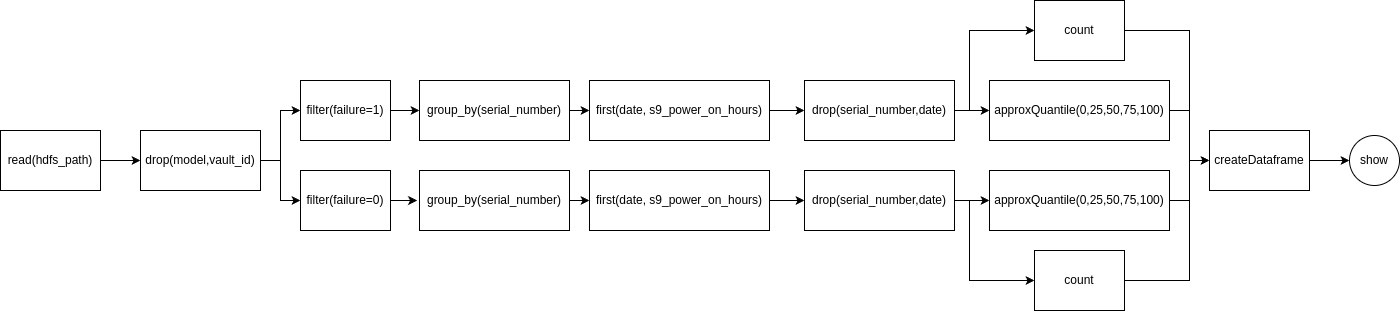
\includegraphics[width=1\textwidth]{res/query3_dag.png}
    \end{adjustbox}
\end{frame}
%----------------------------------------------------------

%-------------------------------------------------------------Slide 13
\subsection{Analytical data storage}
\begin{frame}{Analytical data storage-MongoDB}
    \begin{columns}
    
        \column{0.6\textwidth}
            Per lo storage dei risultati è stato utilizzato \textbf{MongoDB} \\
            \vspace{0.2cm}
            La scrittura da Spark è stata effettuata tramite il \textbf{Spark-MongoDB connector}
        
        \column{0.4\textwidth}
            \begin{minipage}{0.5\textwidth}
                \raggedleft
                
\includegraphics[width=0.8\textwidth]{res/mongodb_icon.png}
            \end{minipage}
    \end{columns}
    \vspace{0.5cm}
    \begin{columns}
        \column{0.5\textwidth}
            \begin{minipage}[b]{1\textwidth}
                Organizzazione dei dati:
                \begin{itemize}
                    \item 1 collezione per ogni query + 1 per performance
                    \item 1 documento per ogni riga
                \end{itemize}
            \end{minipage}
        \column{0.5\textwidth}
            \begin{minipage}{1\textwidth}
                \begin{adjustbox}{margin=0cm 0cm 1.5cm 0cm, center}
                    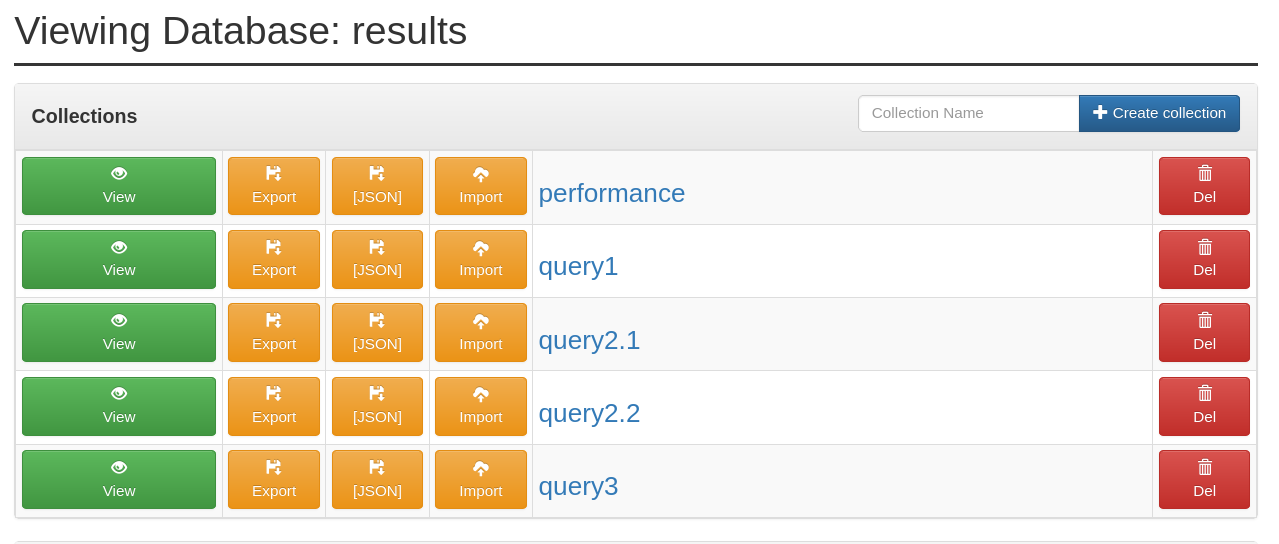
\includegraphics[width=1\textwidth]{res/mongo.png}
                \end{adjustbox}
            \end{minipage}
    \end{columns}
\end{frame}
%----------------------------------------------------------

%---------------------------------------------------------Slide 14
\subsection{Data visualization}
\begin{frame}{Data visualization-Grafana}
    \begin{columns}
        \column{0.6\textwidth}
            Per la visualizzazione dei dati è stato utilizzato \textbf{Grafana}
        \column{0.4\textwidth}
            \begin{minipage}{0.5\textwidth}
                \raggedleft
                
\includegraphics[width=0.8\textwidth]{res/grafana_icon.png}
            \end{minipage}
    \end{columns}
    \vspace{0.5cm}
    \begin{columns}
        \column{0.5\textwidth}
            \begin{minipage}[b]{1\textwidth}
                Pannelli realizzati:
                \begin{itemize}
                    \item 5 pannelli per la visualizzazione dei risultati delle query
                    \item 1 pannello per la visualizzazione delle performance
                \end{itemize}
            \end{minipage}
        \column{0.5\textwidth}
            \begin{minipage}{1\textwidth}
                \begin{adjustbox}{margin=0cm 0cm 1.5cm 0cm, center}
                    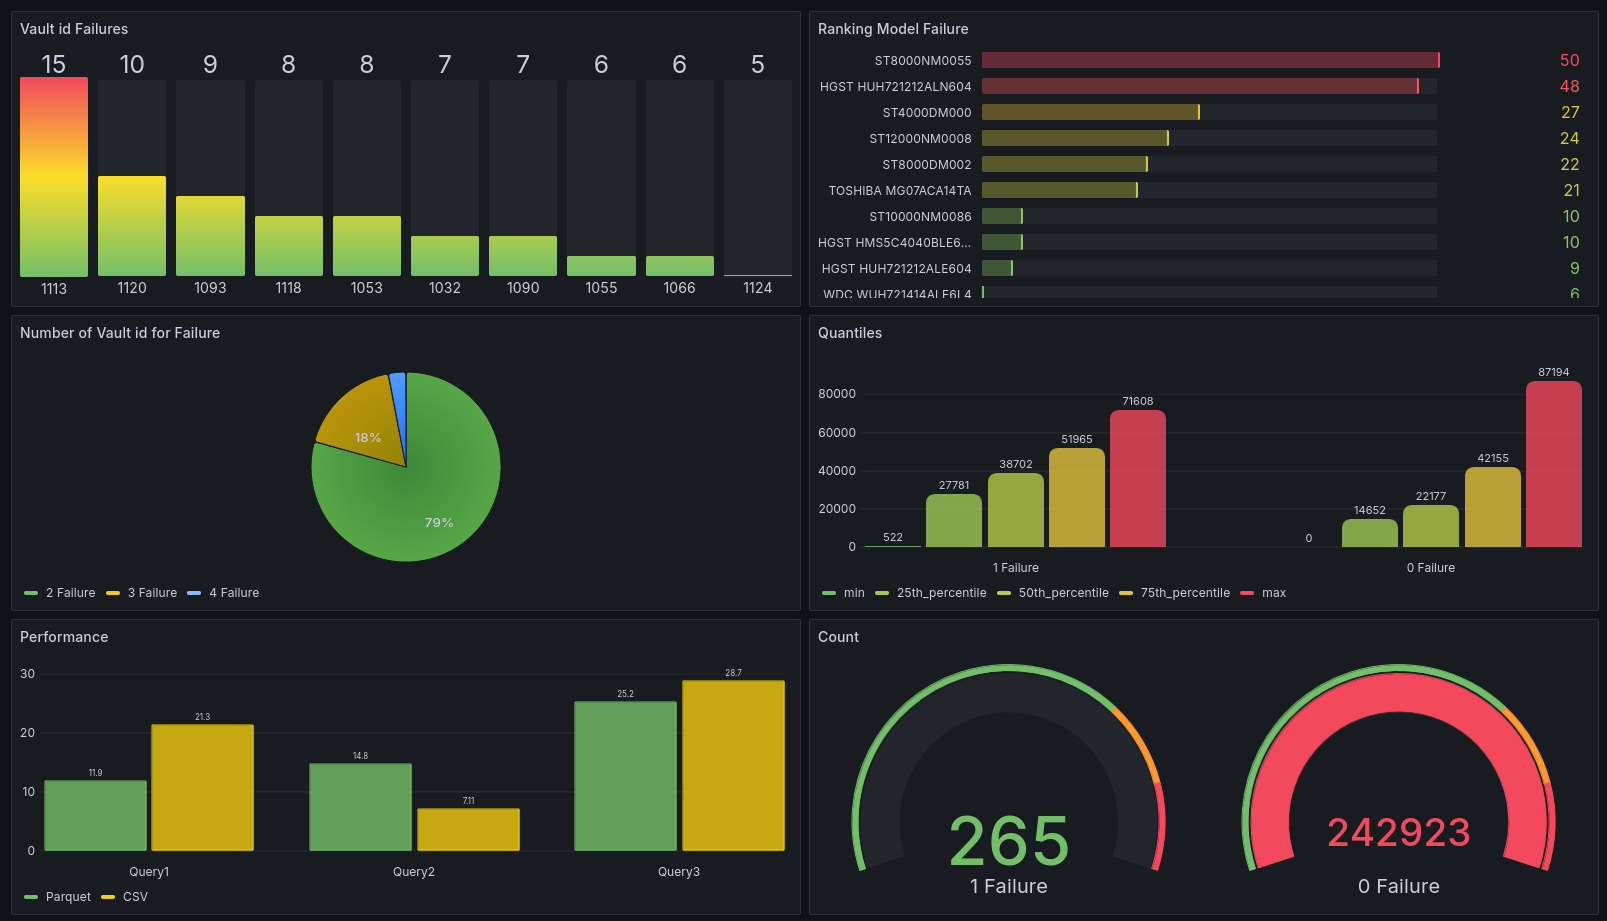
\includegraphics[width=1\textwidth]{res/grafana_dashboard.png}
                \end{adjustbox}
            \end{minipage}
    \end{columns}
\end{frame}
%----------------------------------------------------------

%---------------------CONCLUSIONI---------------------------
\section{Conclusioni}
%---------------------------------------------------------Slide 15
\setLayout{mainpoint}
\setBGColor{TorVergataGreen}
\begin{frame}{}
    \frametitle{Conclusioni}
\end{frame}
%---------------------------------------------------------

\setLayout{vertical}
\subsection{Risultati}
%---------------------------------------------------------Slide 16
\begin{frame}{Risultati-Query1}
    \begin{minipage}{0.9\textwidth}
        \begin{adjustbox}{margin=1cm 0cm 1.5cm 0cm, center}
            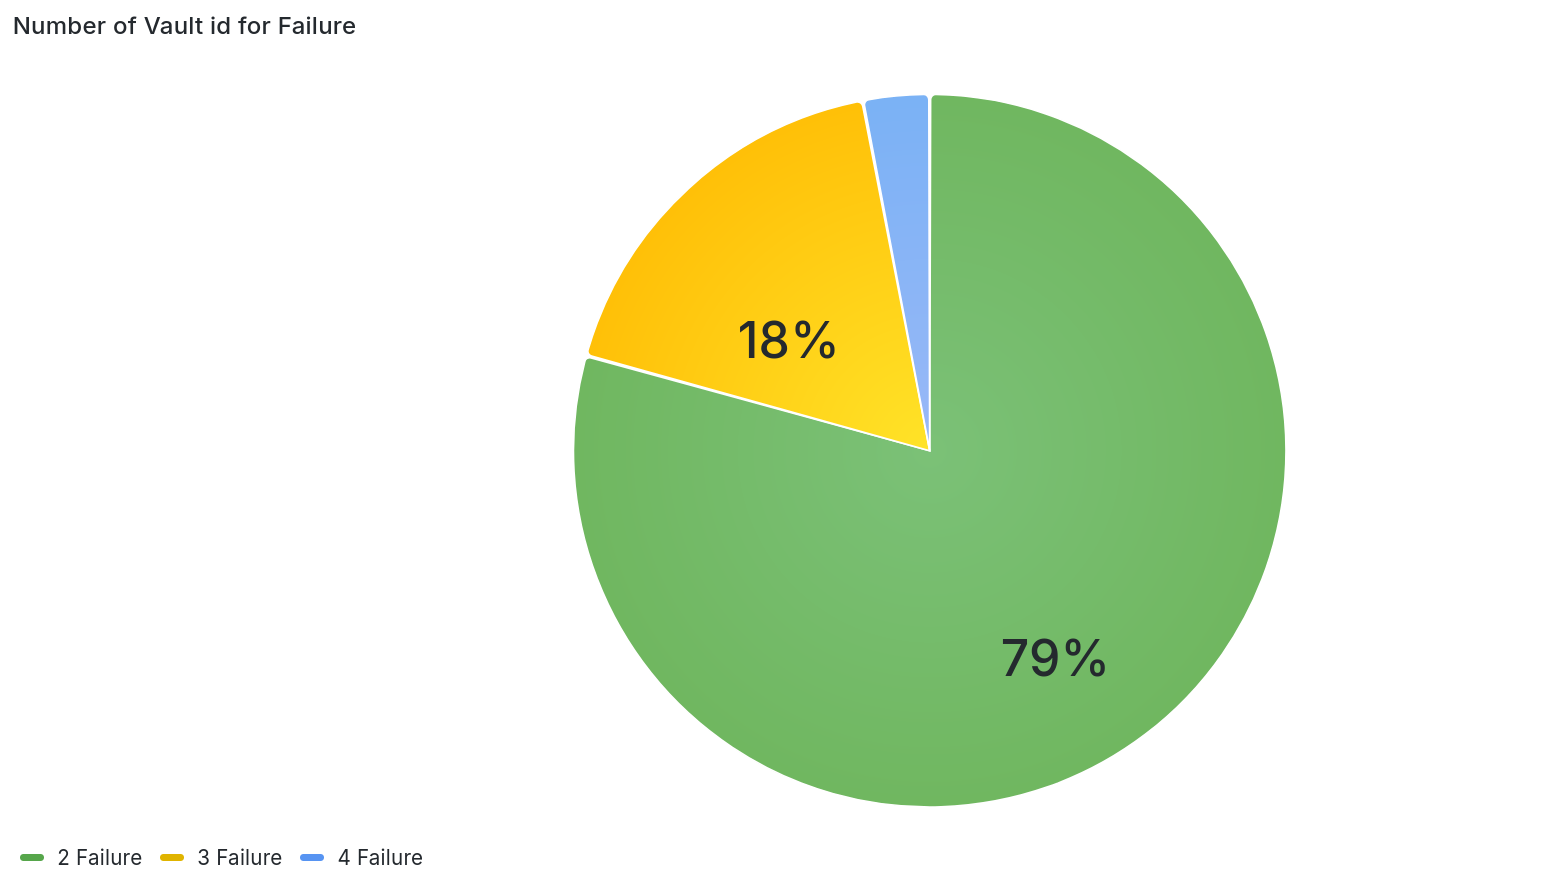
\includegraphics[width=1\textwidth]{res/query1_panel1.png}
        \end{adjustbox}
    \end{minipage}
\end{frame}
%---------------------------------------------------------

%---------------------------------------------------------Slide 17
\begin{frame}{Risultati-Query2}
    \begin{minipage}{0.9\textwidth}
        \begin{adjustbox}{margin=1cm 0cm 1.5cm 0cm, center}
            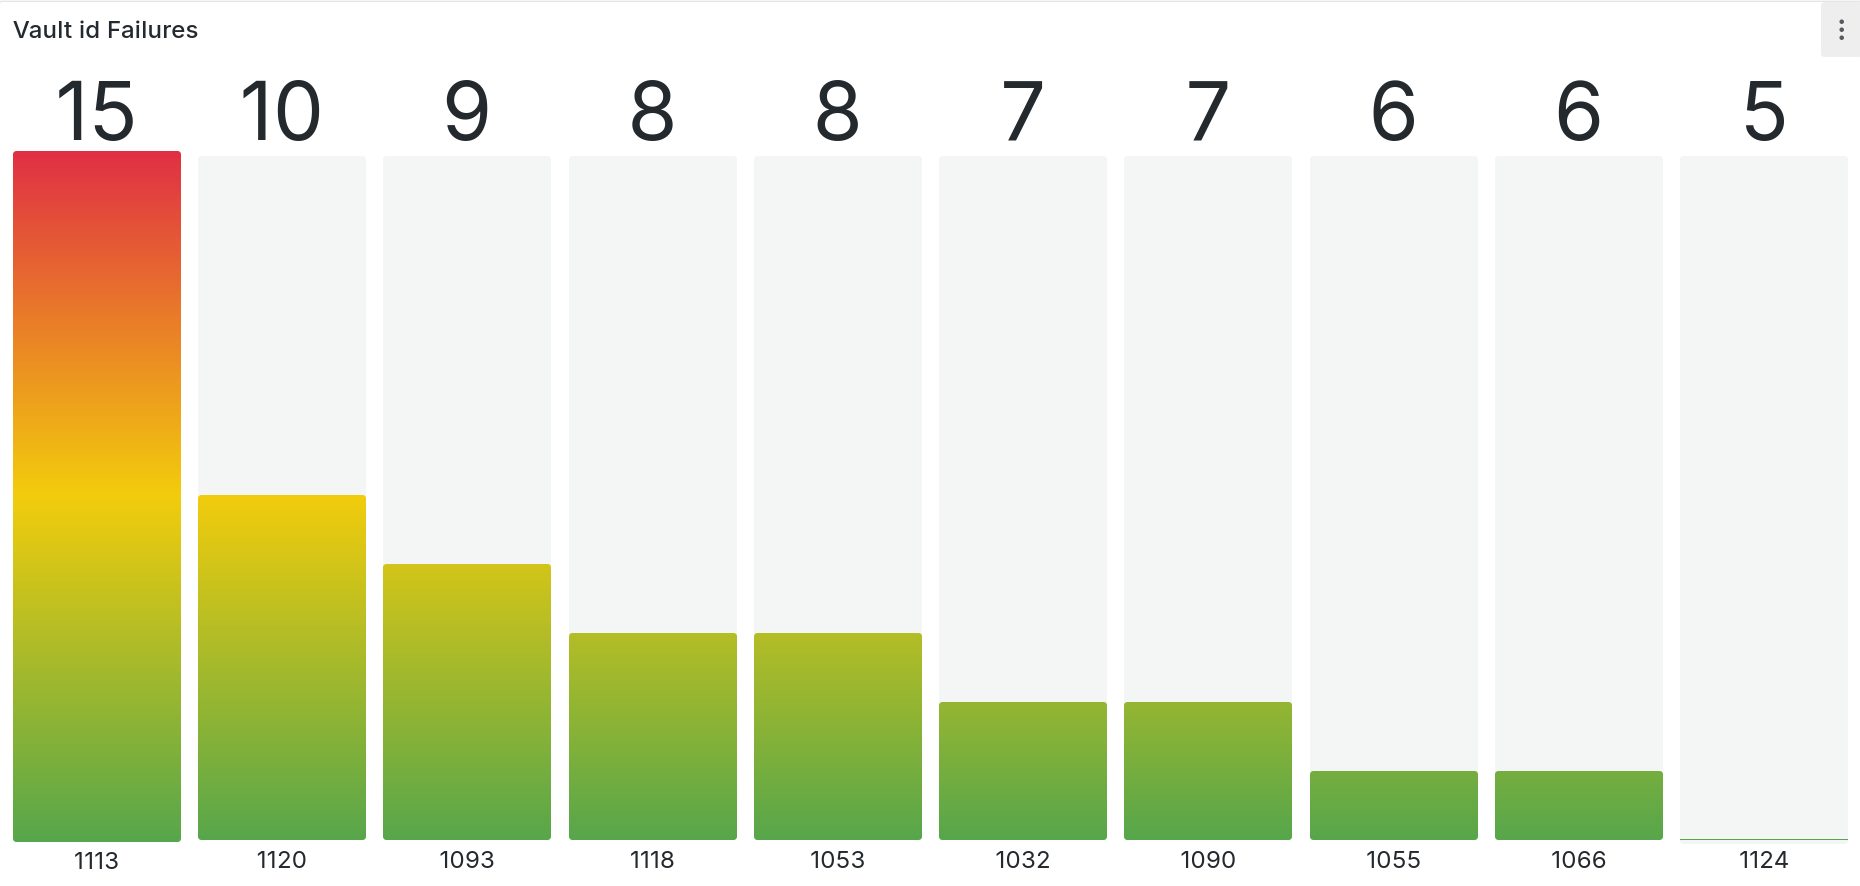
\includegraphics[width=1\textwidth]{res/query2_panel1.png}
        \end{adjustbox}
    \end{minipage}
\end{frame}
%---------------------------------------------------------

%---------------------------------------------------------Slide 18
\begin{frame}{Risultati-Query2}
    \begin{minipage}{0.9\textwidth}
        \begin{adjustbox}{margin=1cm 0cm 1.5cm 0cm, center}
            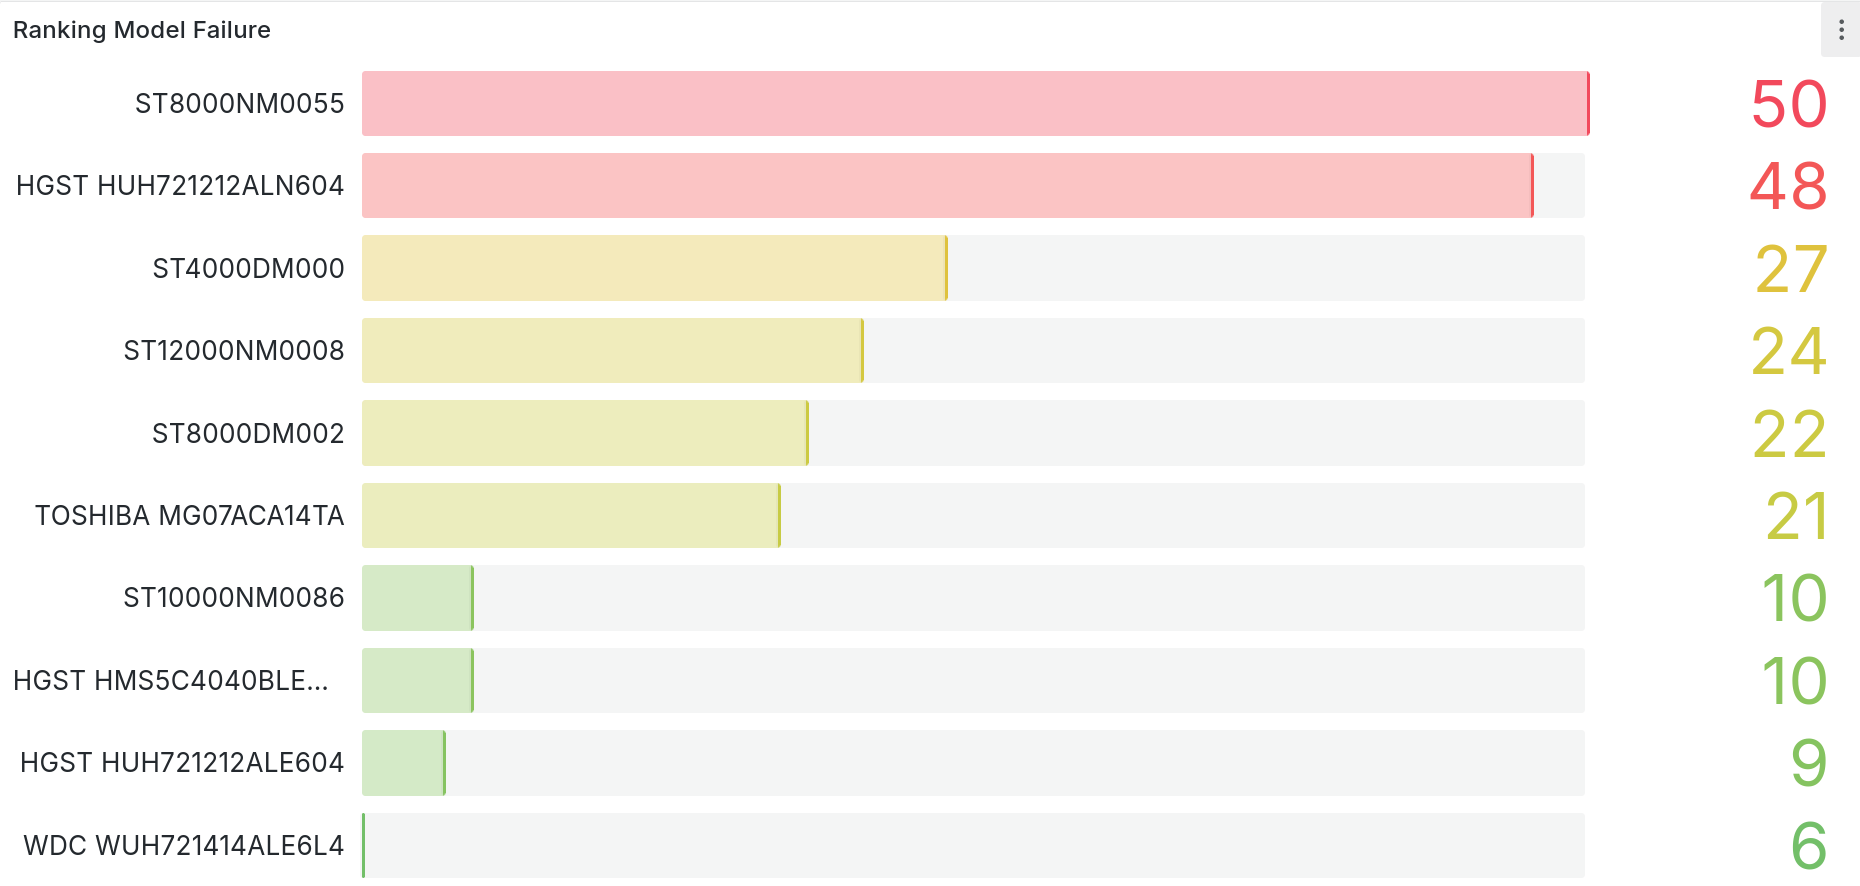
\includegraphics[width=1\textwidth]{res/query2_panel2.png}
        \end{adjustbox}
    \end{minipage}
\end{frame}
%---------------------------------------------------------

%---------------------------------------------------------Slide 19
\begin{frame}{Risultati-Query3}
    \begin{minipage}{0.9\textwidth}
        \begin{adjustbox}{margin=1cm 0cm 1.5cm 0cm, center}
            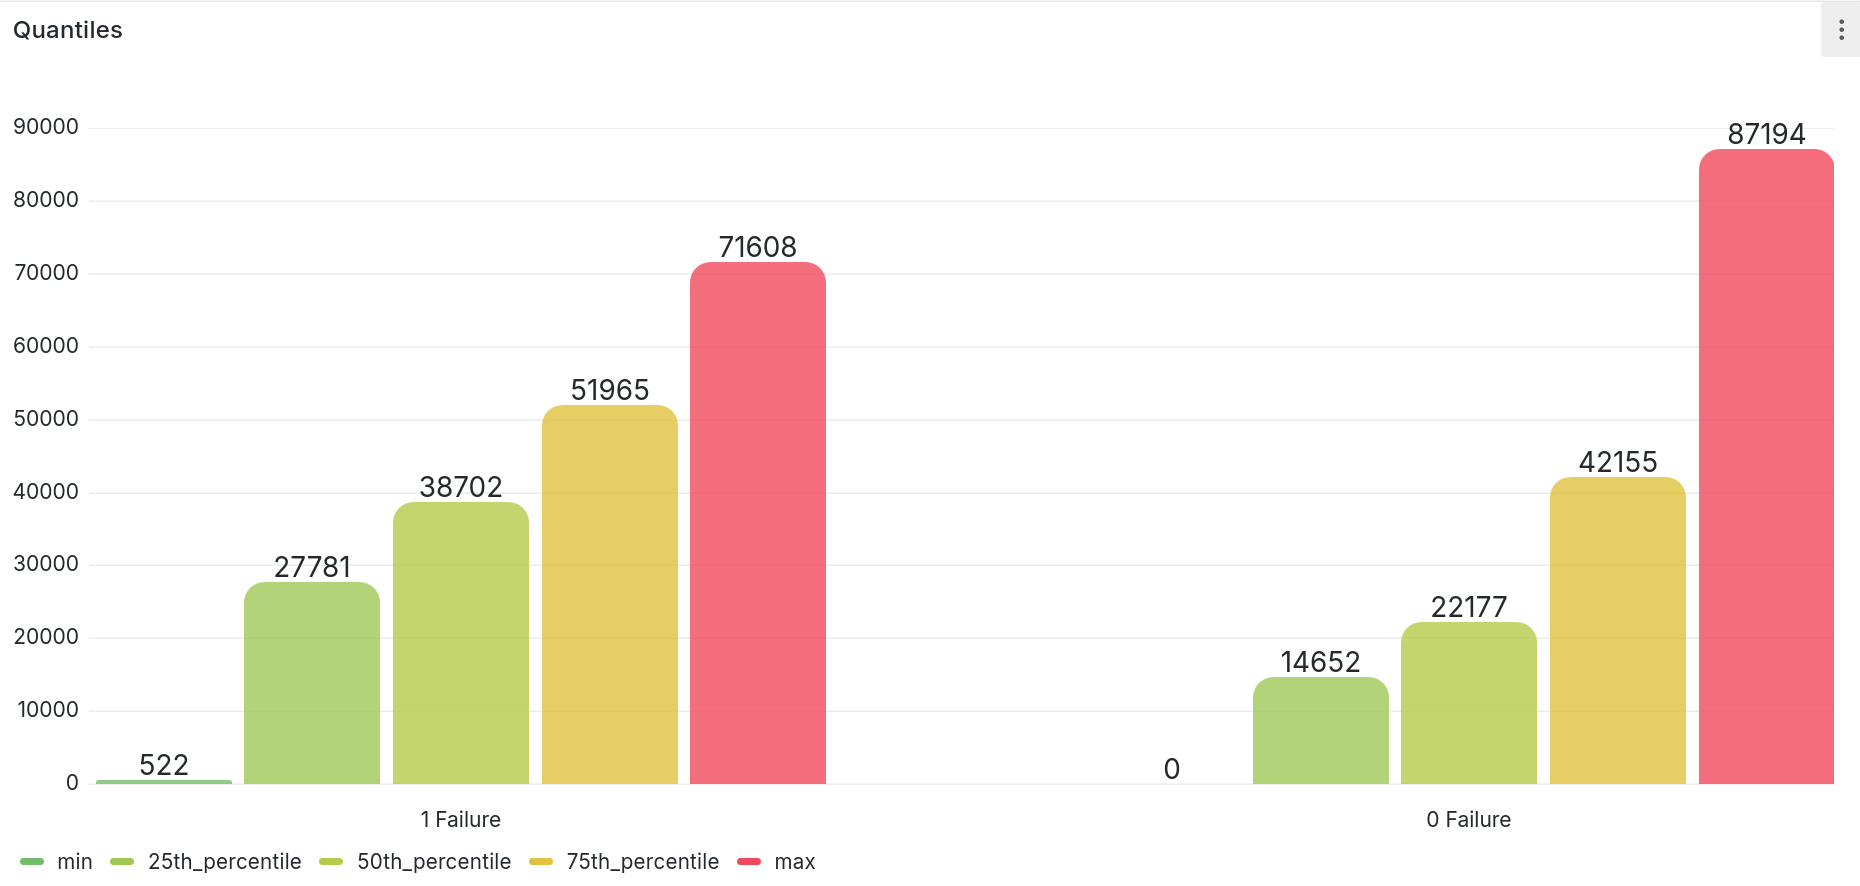
\includegraphics[width=1\textwidth]{res/query3_panel1.png}
        \end{adjustbox}
    \end{minipage}
\end{frame}
%---------------------------------------------------------

%---------------------------------------------------------Slide 20
\begin{frame}{Risultati-Query3}
    \begin{minipage}{0.9\textwidth}
        \begin{adjustbox}{margin=1cm 0cm 1.5cm 0cm, center}
            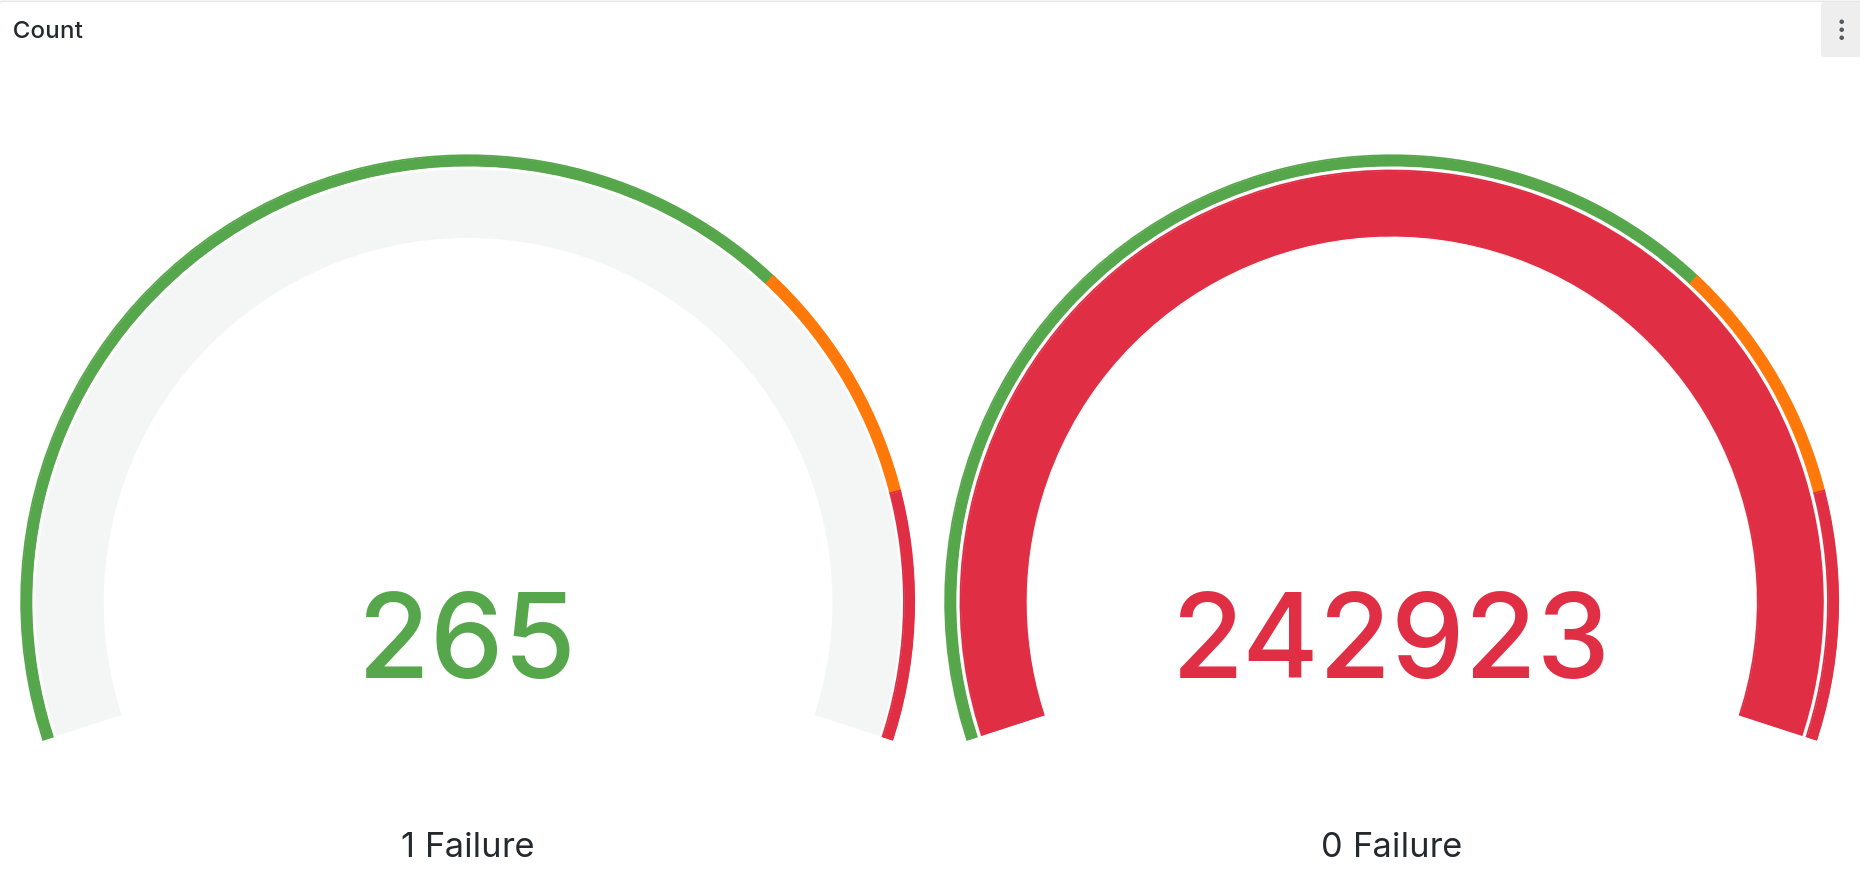
\includegraphics[width=1\textwidth]{res/query3_panel2.png}
        \end{adjustbox}
    \end{minipage}
\end{frame}
%---------------------------------------------------------

\subsection{Performance}
%---------------------------------------------------------Slide 21
\begin{frame}{Performance}
    \begin{minipage}{0.9\textwidth}
        \begin{adjustbox}{margin=0cm 0cm 0cm 0cm, center}
            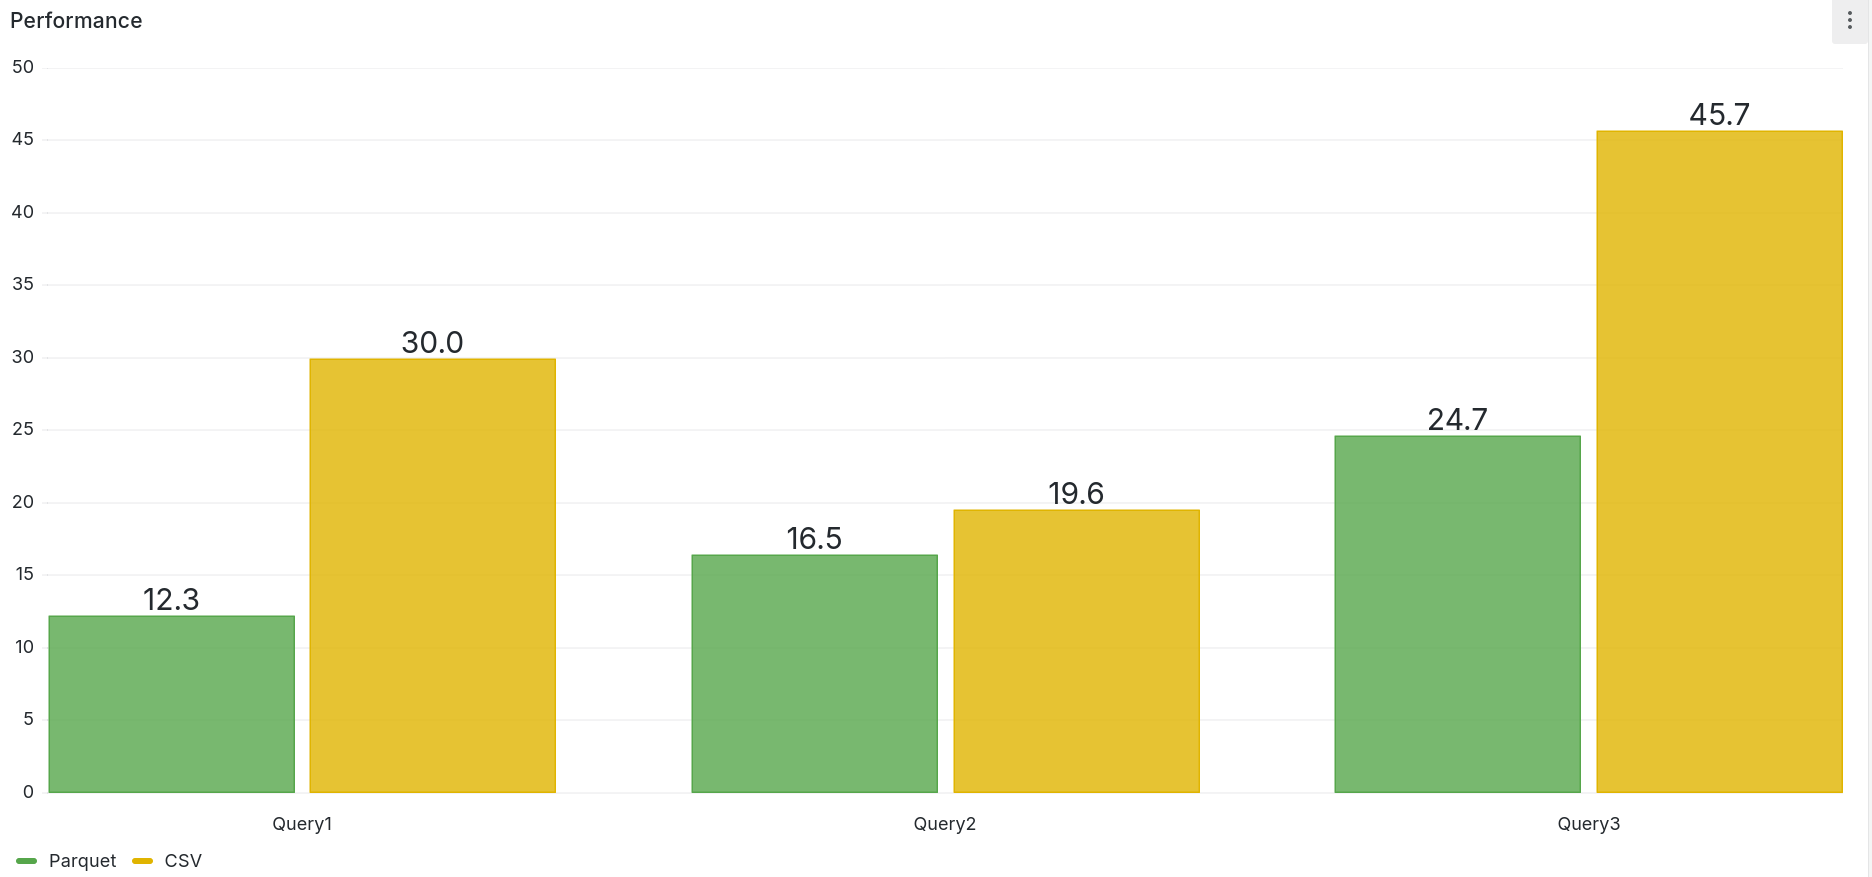
\includegraphics[width=1\textwidth]{res/performance_panel.png}
        \end{adjustbox}
    \end{minipage}
\end{frame}
%---------------------------------------------------------

%---------------------------------------------------------
\setLayout{mainpoint}
\begin{frame}{}
    \frametitle{Grazie per l'attenzione}
\end{frame}
%---------------------------------------------------------
\end{document}